\documentclass[12pt]{article}

\usepackage[english]{babel}
\usepackage[utf8]{inputenc}
\usepackage{amsmath}
\usepackage{commath}
\usepackage{booktabs}
\usepackage[alf]{abntex2cite}
\usepackage{indentfirst}
\usepackage{graphicx}
\usepackage{multicol,lipsum}
\usepackage{geometry}
\usepackage[alf]{abntex2cite}
\usepackage{siunitx}
%\usepackage[scriptsize]{subfigure}
%\usepackage{caption}
\usepackage{subcaption}
\graphicspath{{../../Figures/Report_20_01/}{../../Figures/Report_19_09/}{../../Images/Report_20_01/}}

\geometry{
  paper = a4paper,
  inner = 3cm,
  outer = 3cm,
  top = 2cm,
  bottom = 2cm
}

\usepackage{tabularx}

\renewcommand{\baselinestretch}{1.5} 

\begin{document}
%\maketitle

\begin{titlepage}
\begin{center}

\Huge{Universidade Federal de Alagoas}\\
\large{Instituto de Computação}\\ 
\large{Laboratório de Computação Científica e Análise Numérica}\\ 
\vspace{220pt}
\textbf{\LARGE{Research report}}\\
%\title{{\large{Título}}}
\vspace{3,5cm}
\end{center}

\begin{flushleft}
\begin{tabbing}
Student: Danilo Fernandes Costa\\
Professor: Alejandro Frery\\
\end{tabbing}
\end{flushleft}
\vspace{1cm}

\begin{center}
\vspace{\fill}
January\\
2020
\end{center}
\end{titlepage}

\section{Introduction}

In this report, we analyse five PolSAR images of the same region -- a soilbeans crop -- obtained over time, which were disponibilized by Avik Bhattacharya and his research group. The first image was made on 16 May 2016, which was followed by four others at time intervals of 24 days. These images have the dimensions $30 \times 65$ and are shown in the figures \ref{fig:day_0} to \ref{fig:day_96} through Pauli Decomposition. 

\begin{figure}[hbt]
  \centering
  \subcaptionbox{16 May 2016\label{fig:day_0}}{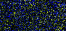
\includegraphics[width = .19\linewidth]{sb231_day_0}}
  \subcaptionbox{09 June 2016\label{fig:day_24}}{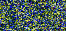
\includegraphics[width = .19\linewidth]{sb231_day_24}}
  \subcaptionbox{03 July 2016\label{fig:day_48}}{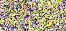
\includegraphics[width = .19\linewidth]{sb231_day_48}}
  \subcaptionbox{27 July 2016\label{fig:day_72}}{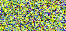
\includegraphics[width = .19\linewidth]{sb231_day_72}}
  \subcaptionbox{20 Aug. 2016\label{fig:day_96}}{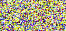
\includegraphics[width = .19\linewidth]{sb231_day_96}}
  \caption{Sample analyzed over time}
  \label{fig:sample_images}
\end{figure}

The roadmap for the data analysis of these images followed as follows:
\begin{itemize}
  \item Obtaining the geodesic purity index and scattering type angle of the data;
  \item Descriptive analysis of the data by image through histograms and boxplots;
  \item Fitting of histograms to known probability distributions;
  \item Separability test.
\end{itemize}

The geodesic purity index measures the distance between a target and the ideal depolarizer. This is, as a Kennaugh matrix, given by:

{\setstretch{1.0}
\[ \mathbf{K}_{dep} =
\begin{bmatrix}
1 & 0 & 0 & 0\\
0 & 0 & 0 & 0\\
0 & 0 & 0 & 0\\
0 & 0 & 0 & 0
\end{bmatrix}.
\]
}
The geodesic purity index is calculated as follows:
\begin{equation}
  P_{GD} = \left(\frac{3}{2}GD(\mathbf{K}, \mathbf{K}_{dep})\right)^2
\end{equation}

\section{Data analysis}

\subsection{Geodesic Purity Index}

After calculating the purity for the analyzed dataset, histograms and boxplots were obtained from the logarithm of the calculated indices for each image, which are shown in the figure \ref{fig:histograms_purity}. Through this graph, one can suppose that these data obey a Normal distribution. To graphically analyze this, the respective qqplots were produced, which are shown in the figure \ref{fig:qqplots}. It can be seen that these graphs are compliant with the supposition.

\begin{figure}[hbt]
  \centering
  \subcaptionbox{Histograms\label{fig:histograms_purity}}{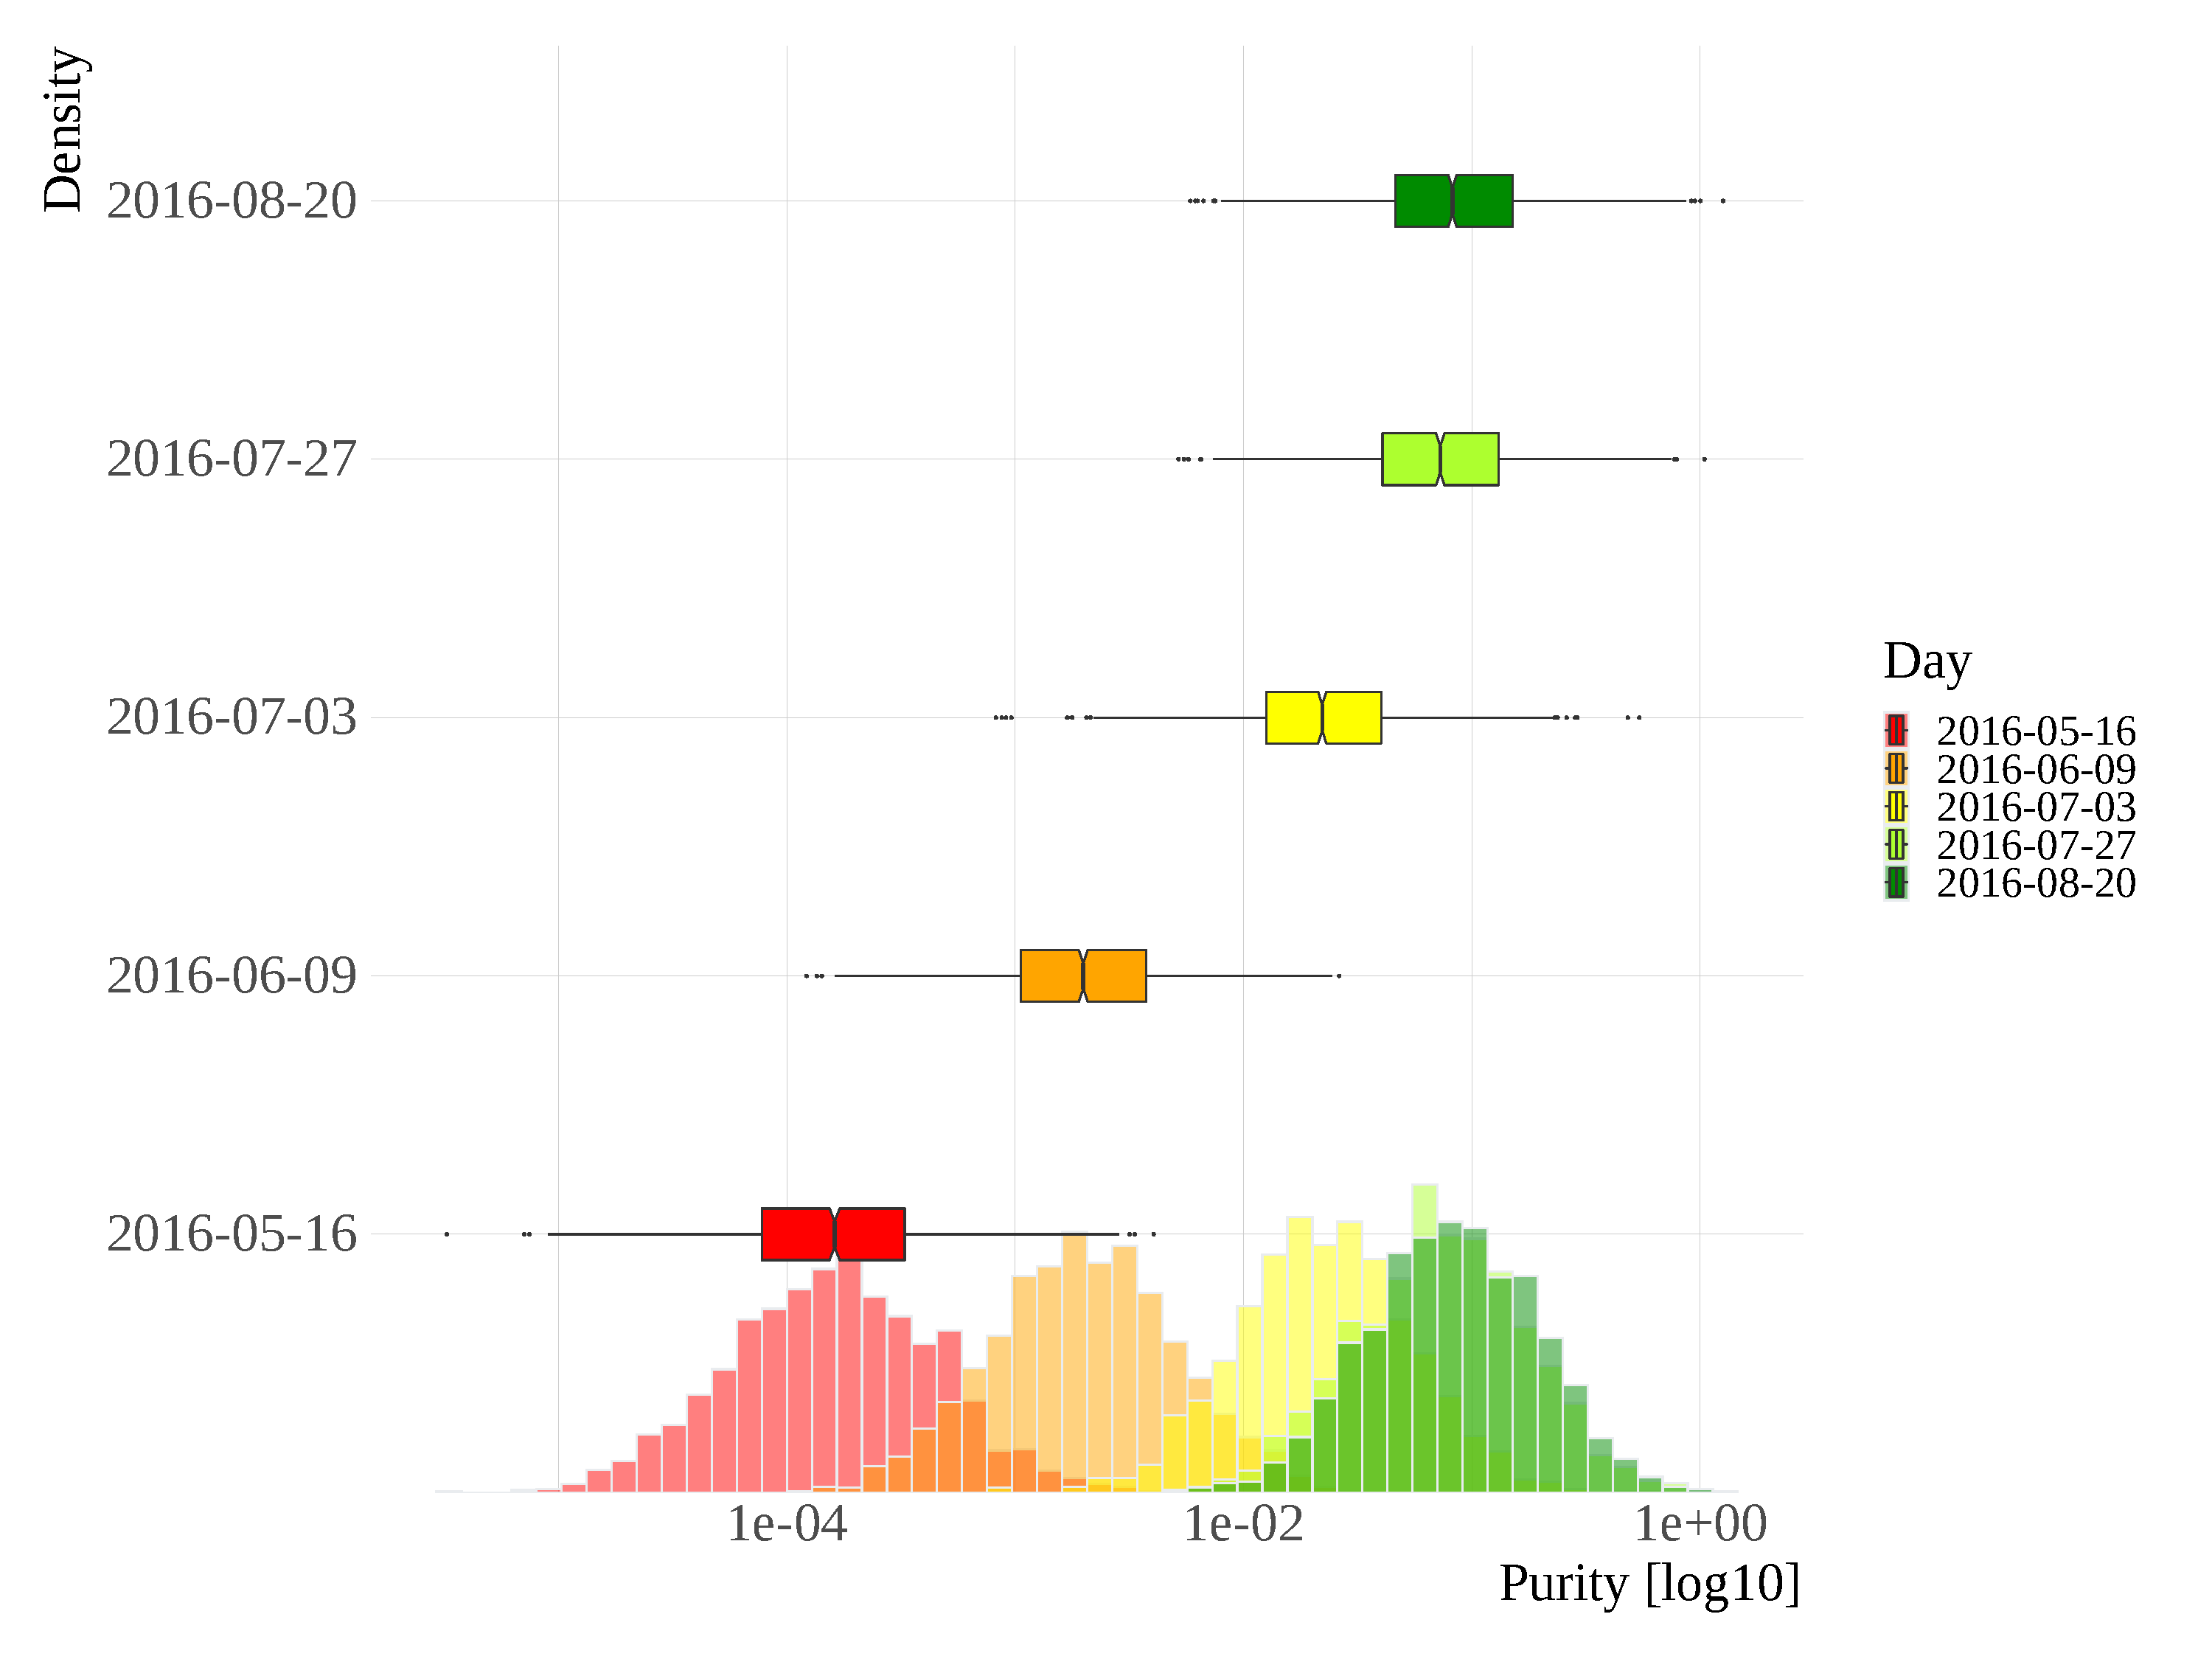
\includegraphics[width = .495\linewidth]{histograms}}
  \subcaptionbox{QQPlots\label{fig:qqplots}}{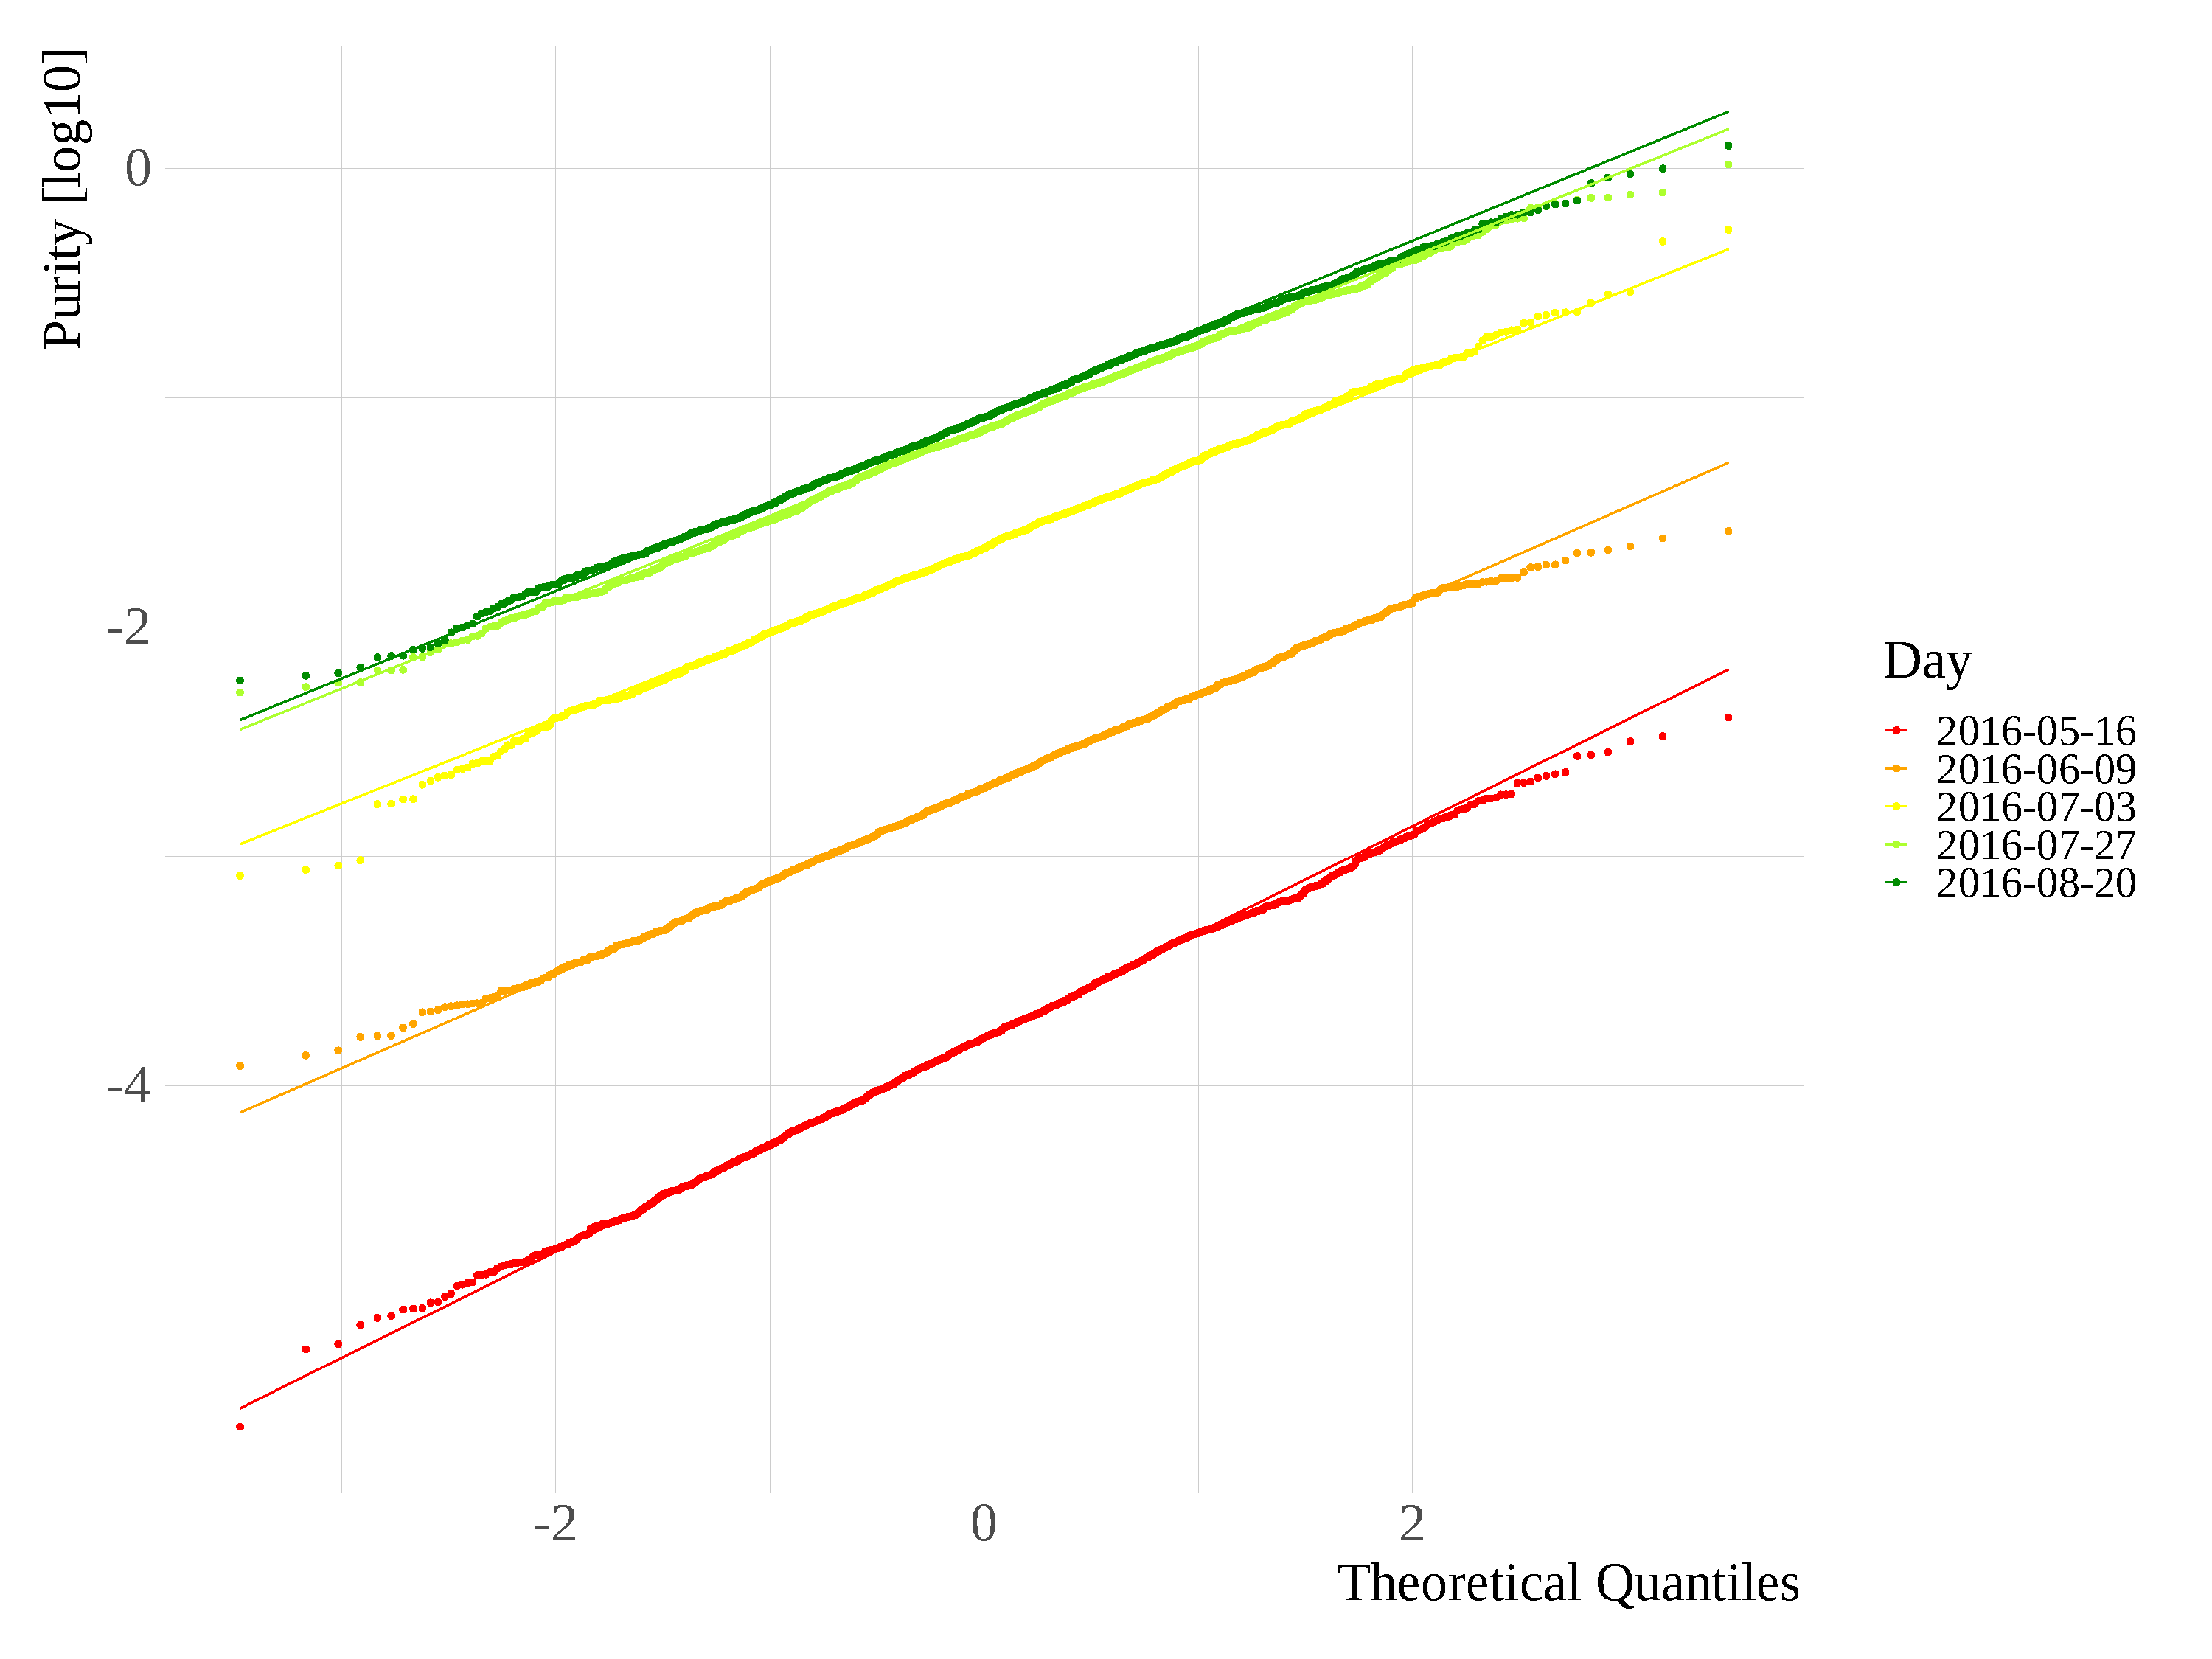
\includegraphics[width = .495\linewidth]{qqplots}}
  \caption{Descriptive analysis of the logarithm of the calculated purity values for each image}
  \label{fig:desc_analysis}
\end{figure}

Based on this assumption, normality tests (Shapiro-Wilk test) were performed from which the $p$-values are in the table \ref{tab:pvalues_purities}. From these, it is possible to conclude that, at the level of $0.05$, it is not possible to reject the null hypothesis that these data obey the Normal distribution. 

\begin{table}[hbt]
  \centering
  \caption{$p$-values from Shapiro-Wilk Test}
  \label{tab:pvalues_purities}
  \begin{tabular}{lrrrrr}
    \toprule
    \textbf{Day} & \textbf{16 May} & \textbf{09 June} & \textbf{03 July} & \textbf{27 July} & \textbf{20 Aug.}\\
                 & \textbf{2016} & \textbf{2016} & \textbf{2016} & \textbf{2016} & \textbf{2016}\\
    \textbf{$p$-value} & 0.4963 & 0.0650 & 0.3494 & 0.0585 & 0.3919\\
    \bottomrule
  \end{tabular}
\end{table}

\subsection{Geodesic Scattering Type Angle}

In this analysis, the geodetic distance to the trihedral - the normalized geodesic scattering type angle - was obtained from the samples. From these computed distances, those referring to pixels closer to the trihedral than to the other elementary scatterers (cylinder, dipole, dihedral, narrow dihedral, left helix, right helix, $-1/4$-wave, $+1/4$-wave) were selected.

From this selected distances per image, it was generated the histograms shown in the figure \ref{fig:histograms_alpha}. Through these graphs, one can suppose that these data obey a Beta distribution. To evaluate this assumption, the Komolgorov-Smirnov test was performed, whose $p$-values are in the table \ref{tab:pvalues_alpha} along with the sample size.

\begin{figure}[hbt]
\centering
\subcaptionbox{16 May 2016}{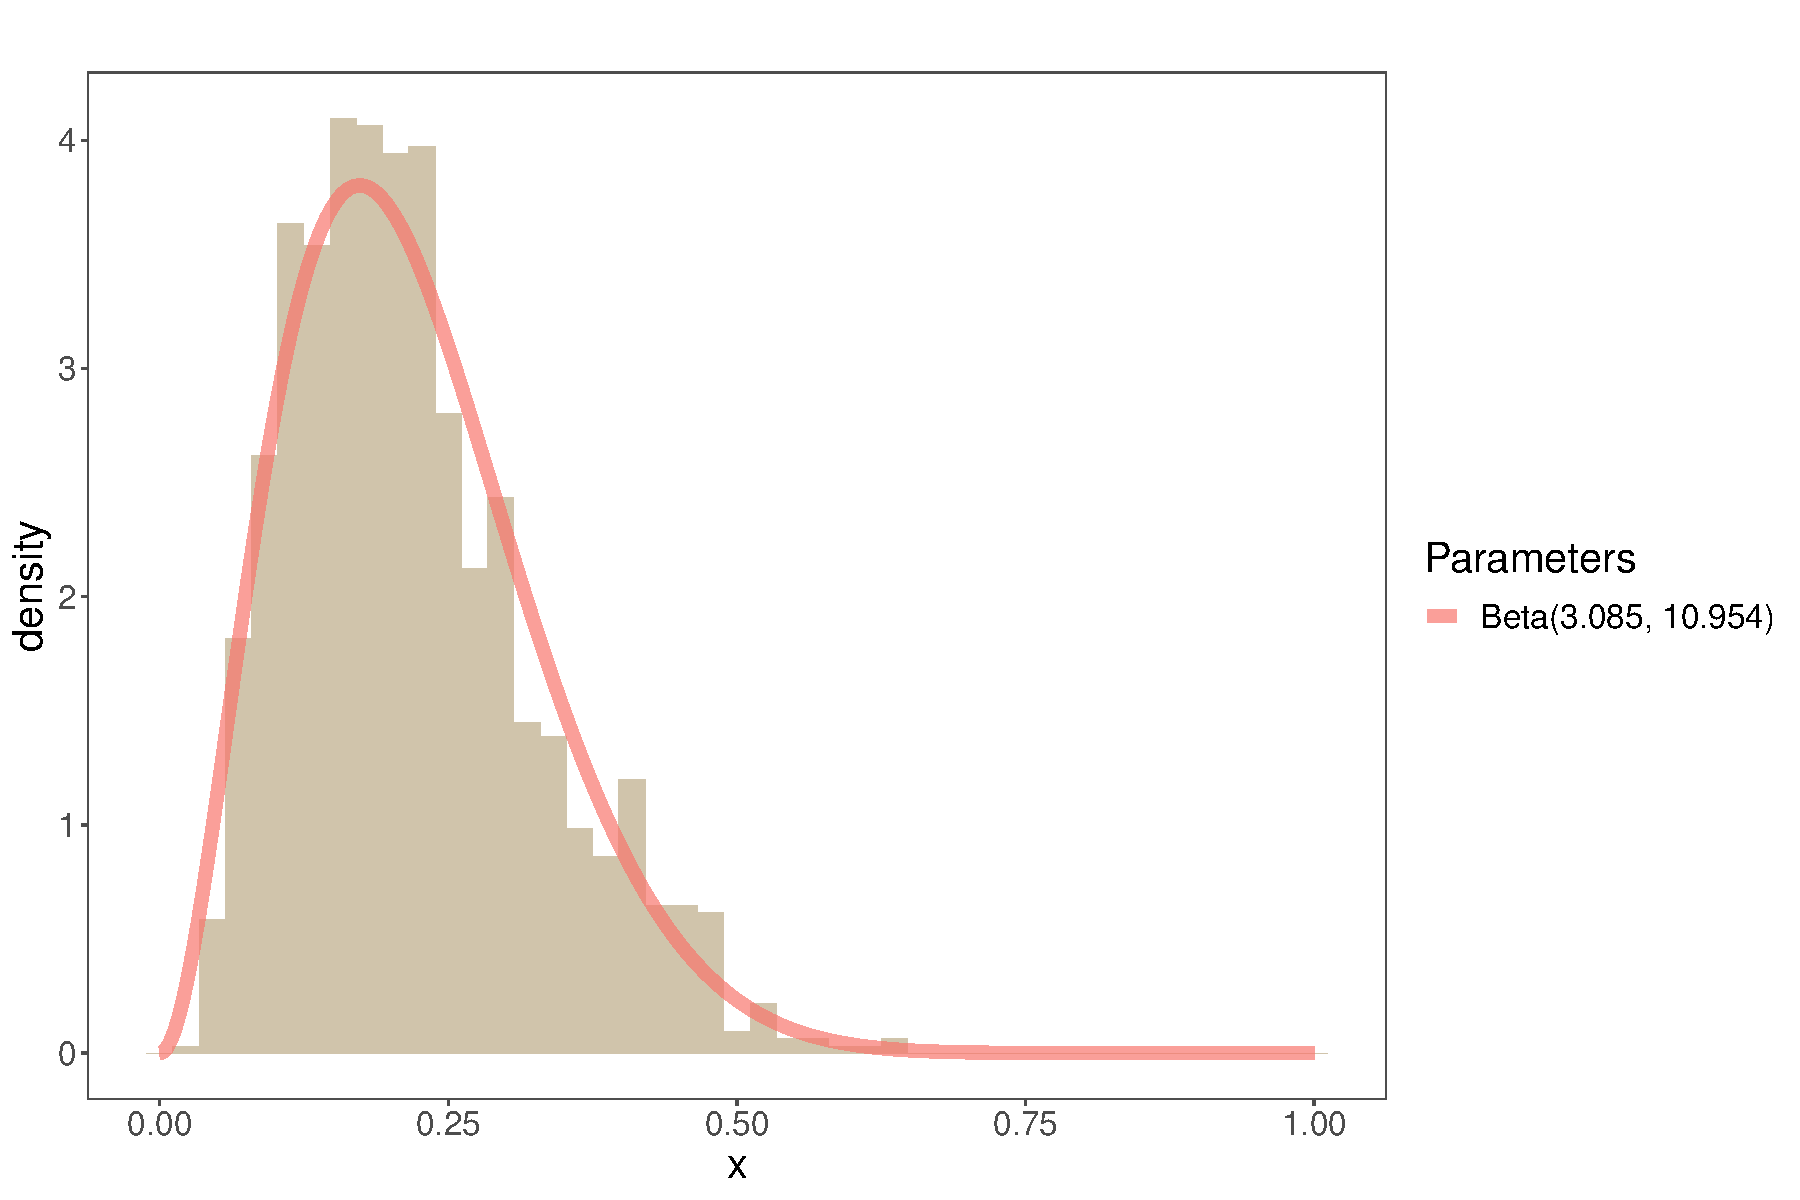
\includegraphics[width = .19\linewidth]{/Histograms/1th_observation/Soybeans_231/histogram_trihedral_1}}
\subcaptionbox{09 June 2016}{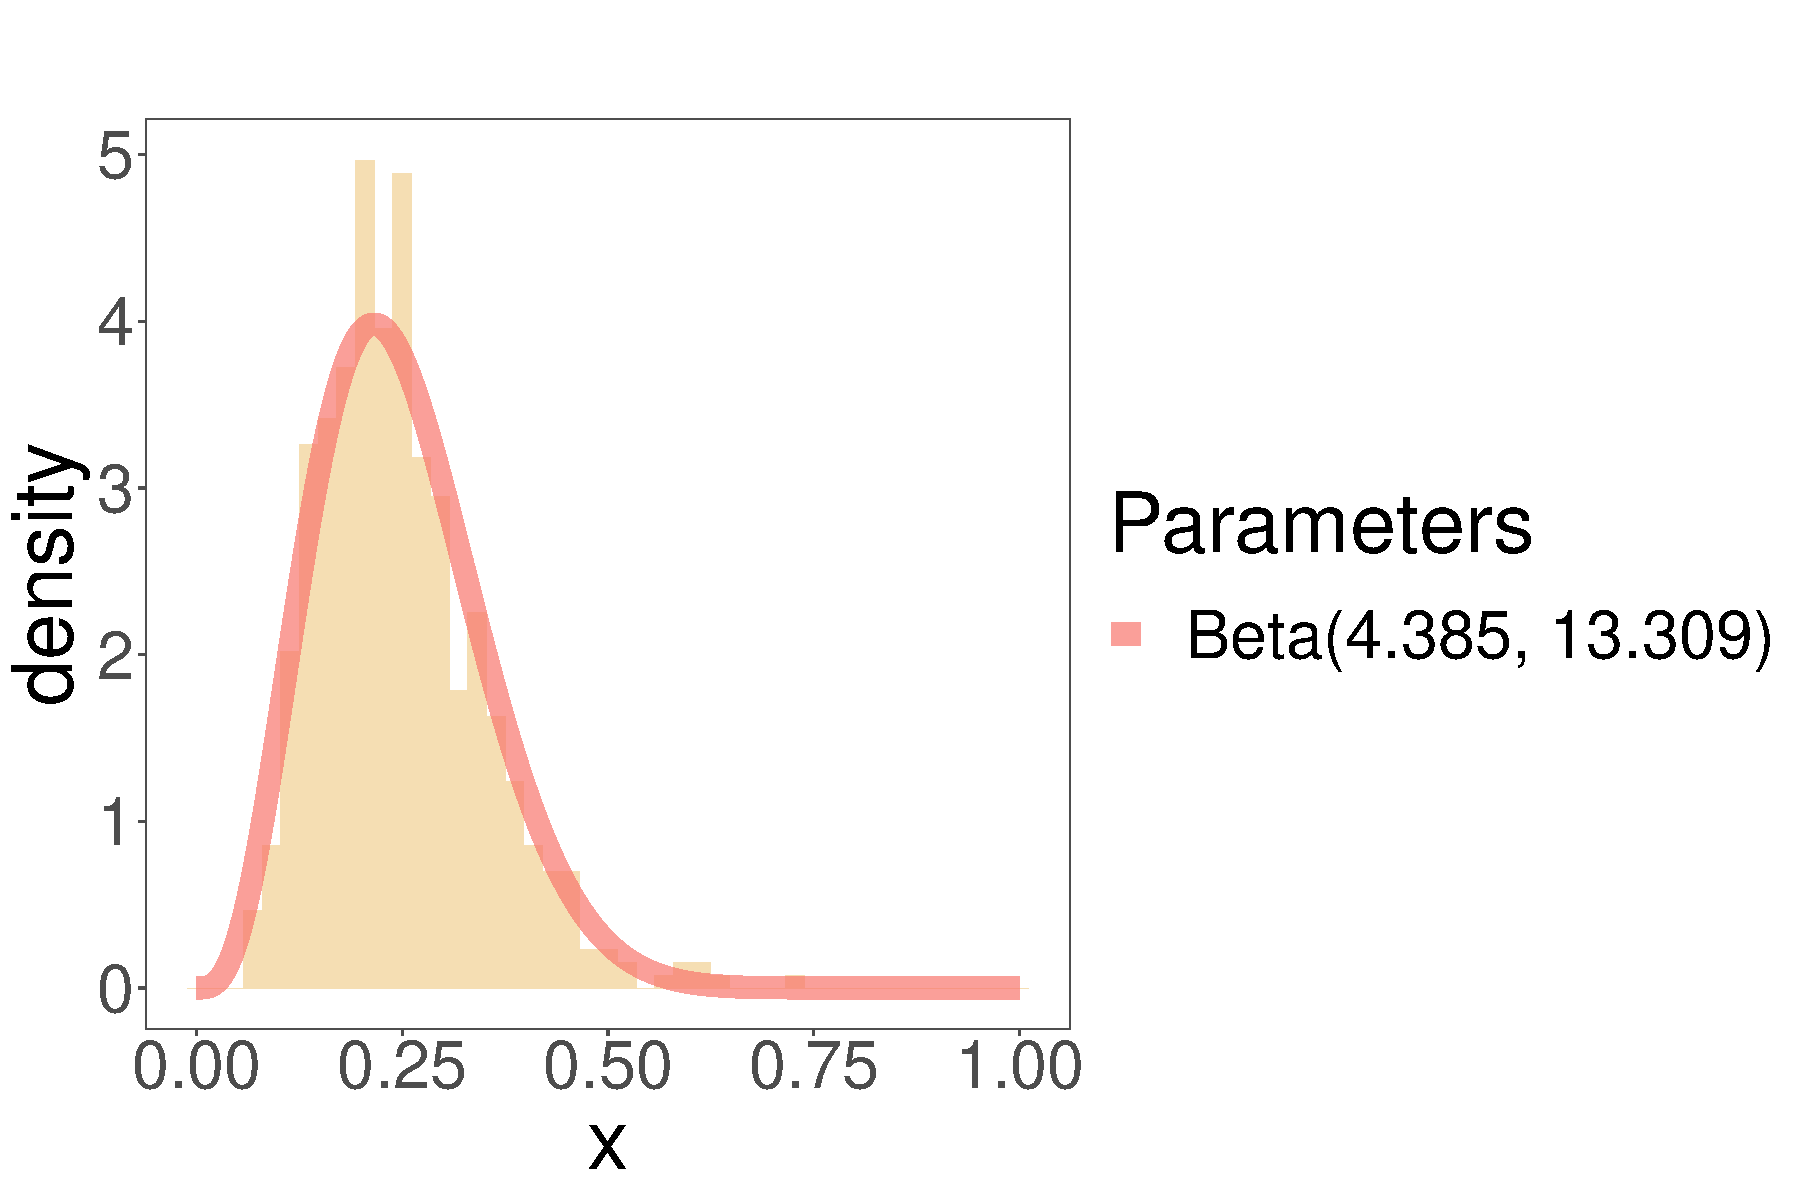
\includegraphics[width = .19\linewidth]{/Histograms/2th_observation/Soybeans_231/histogram_trihedral_2}}
\subcaptionbox{03 July 2016}{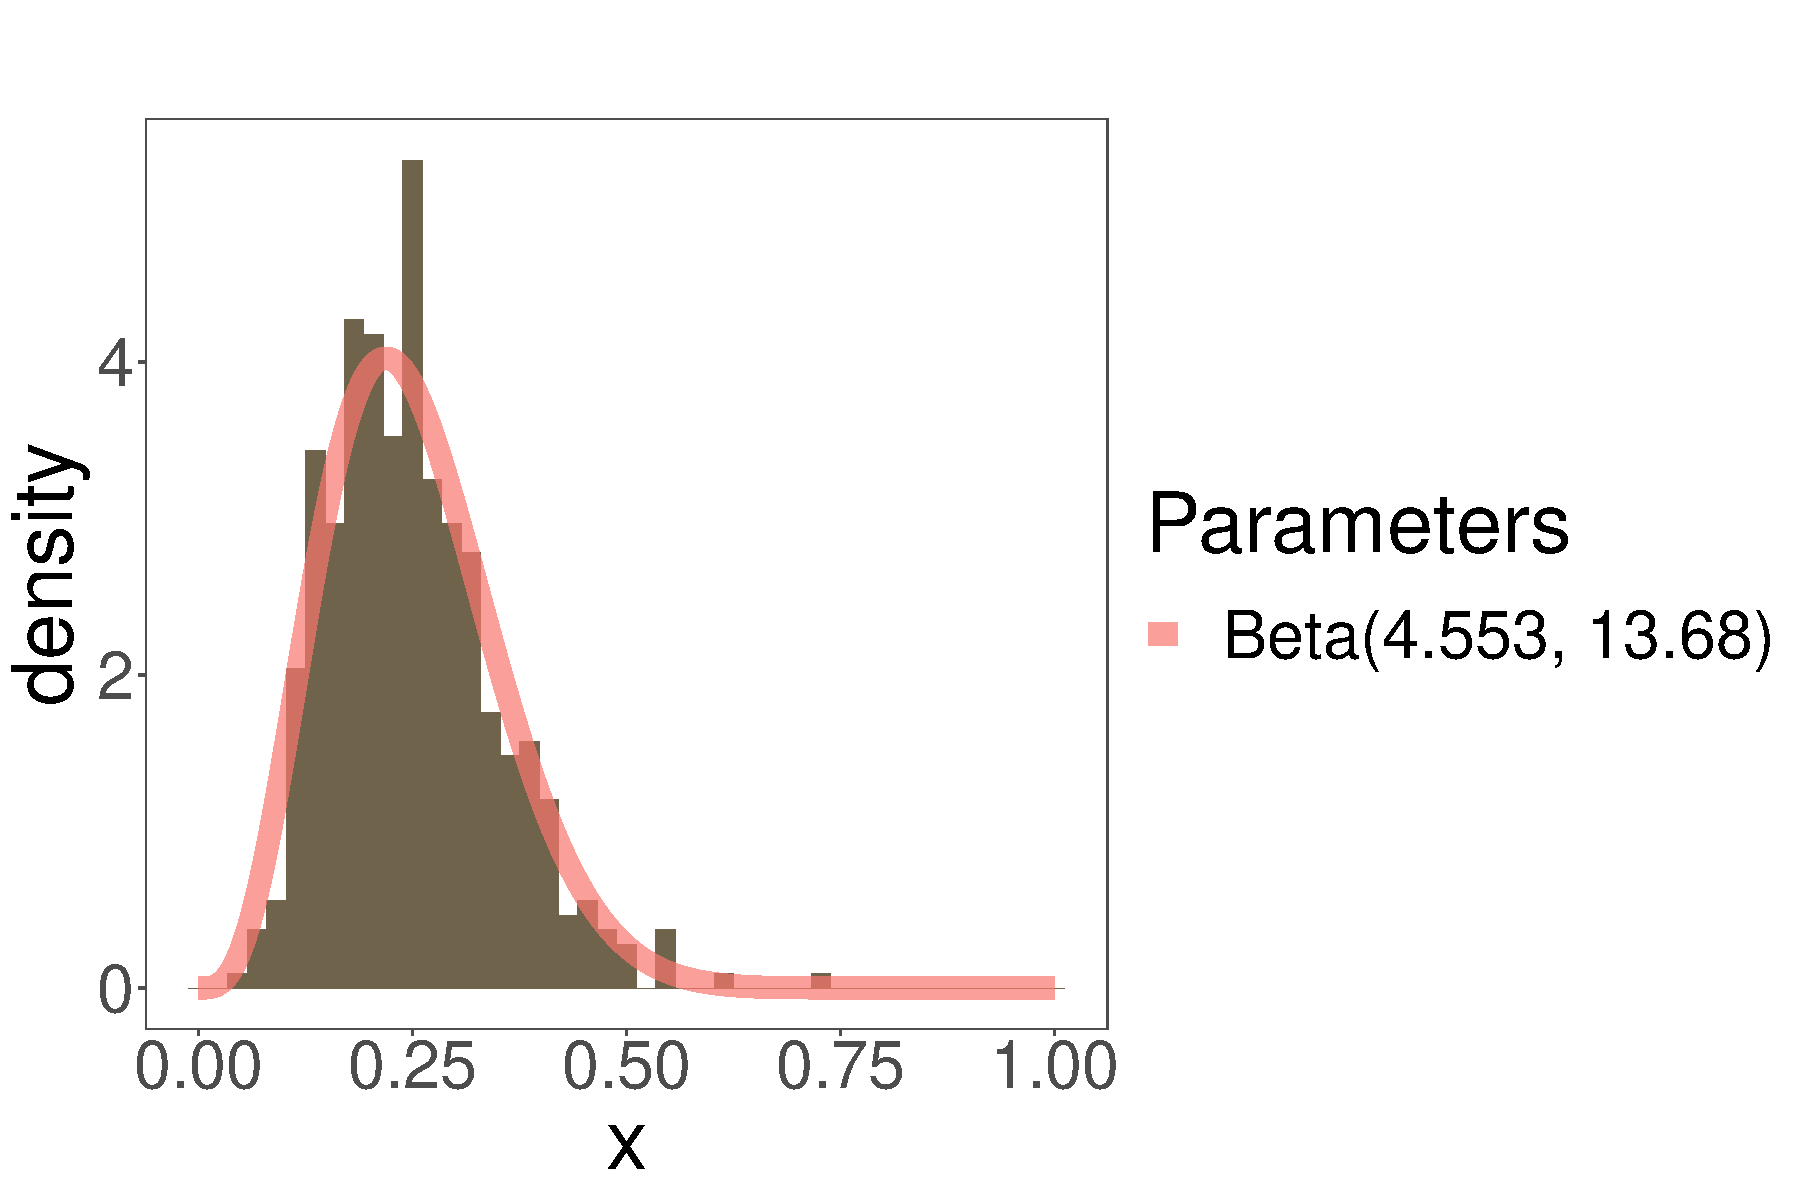
\includegraphics[width = .19\linewidth]{/Histograms/3th_observation/Soybeans_231/histogram_trihedral_3}}
\subcaptionbox{27 July 2016}{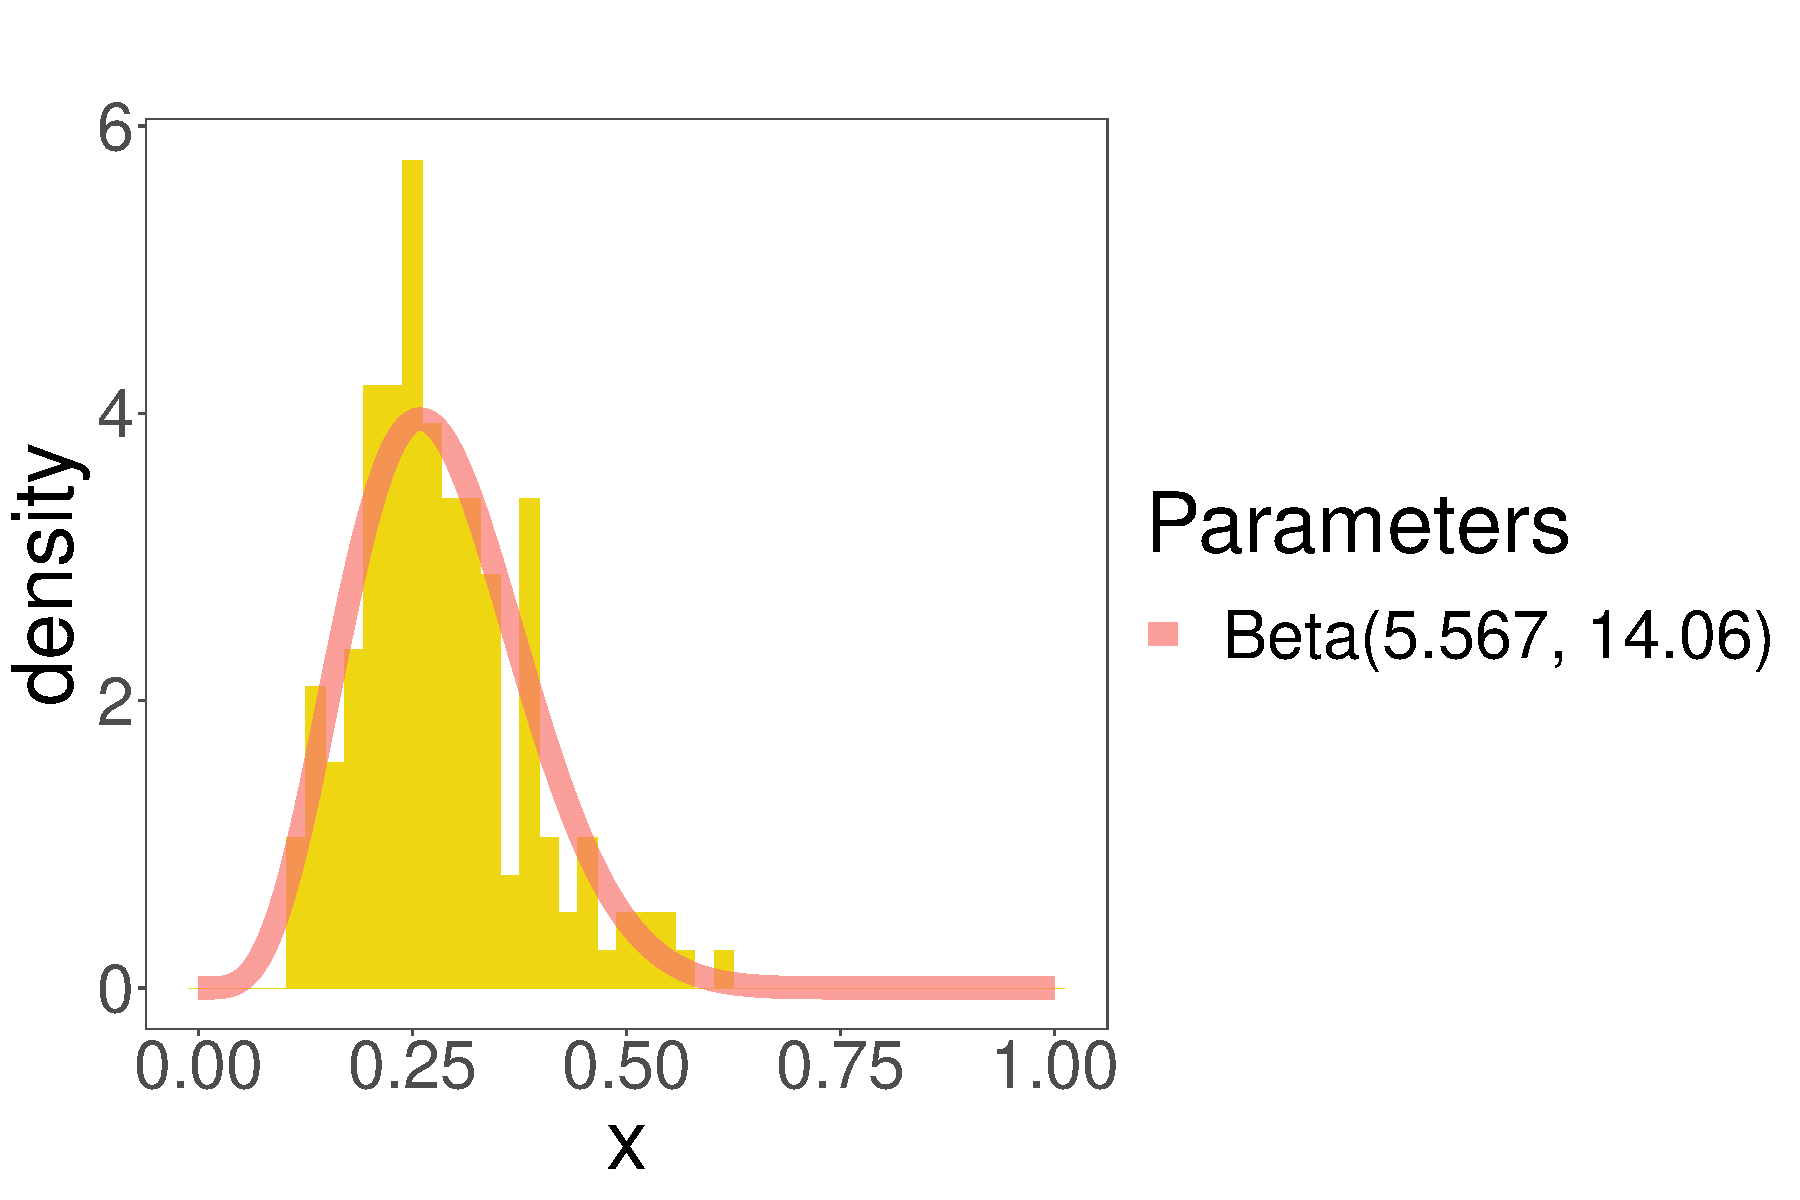
\includegraphics[width = .19\linewidth]{/Histograms/4th_observation/Soybeans_231/histogram_trihedral_4}}
\subcaptionbox{20 Aug. 2016}{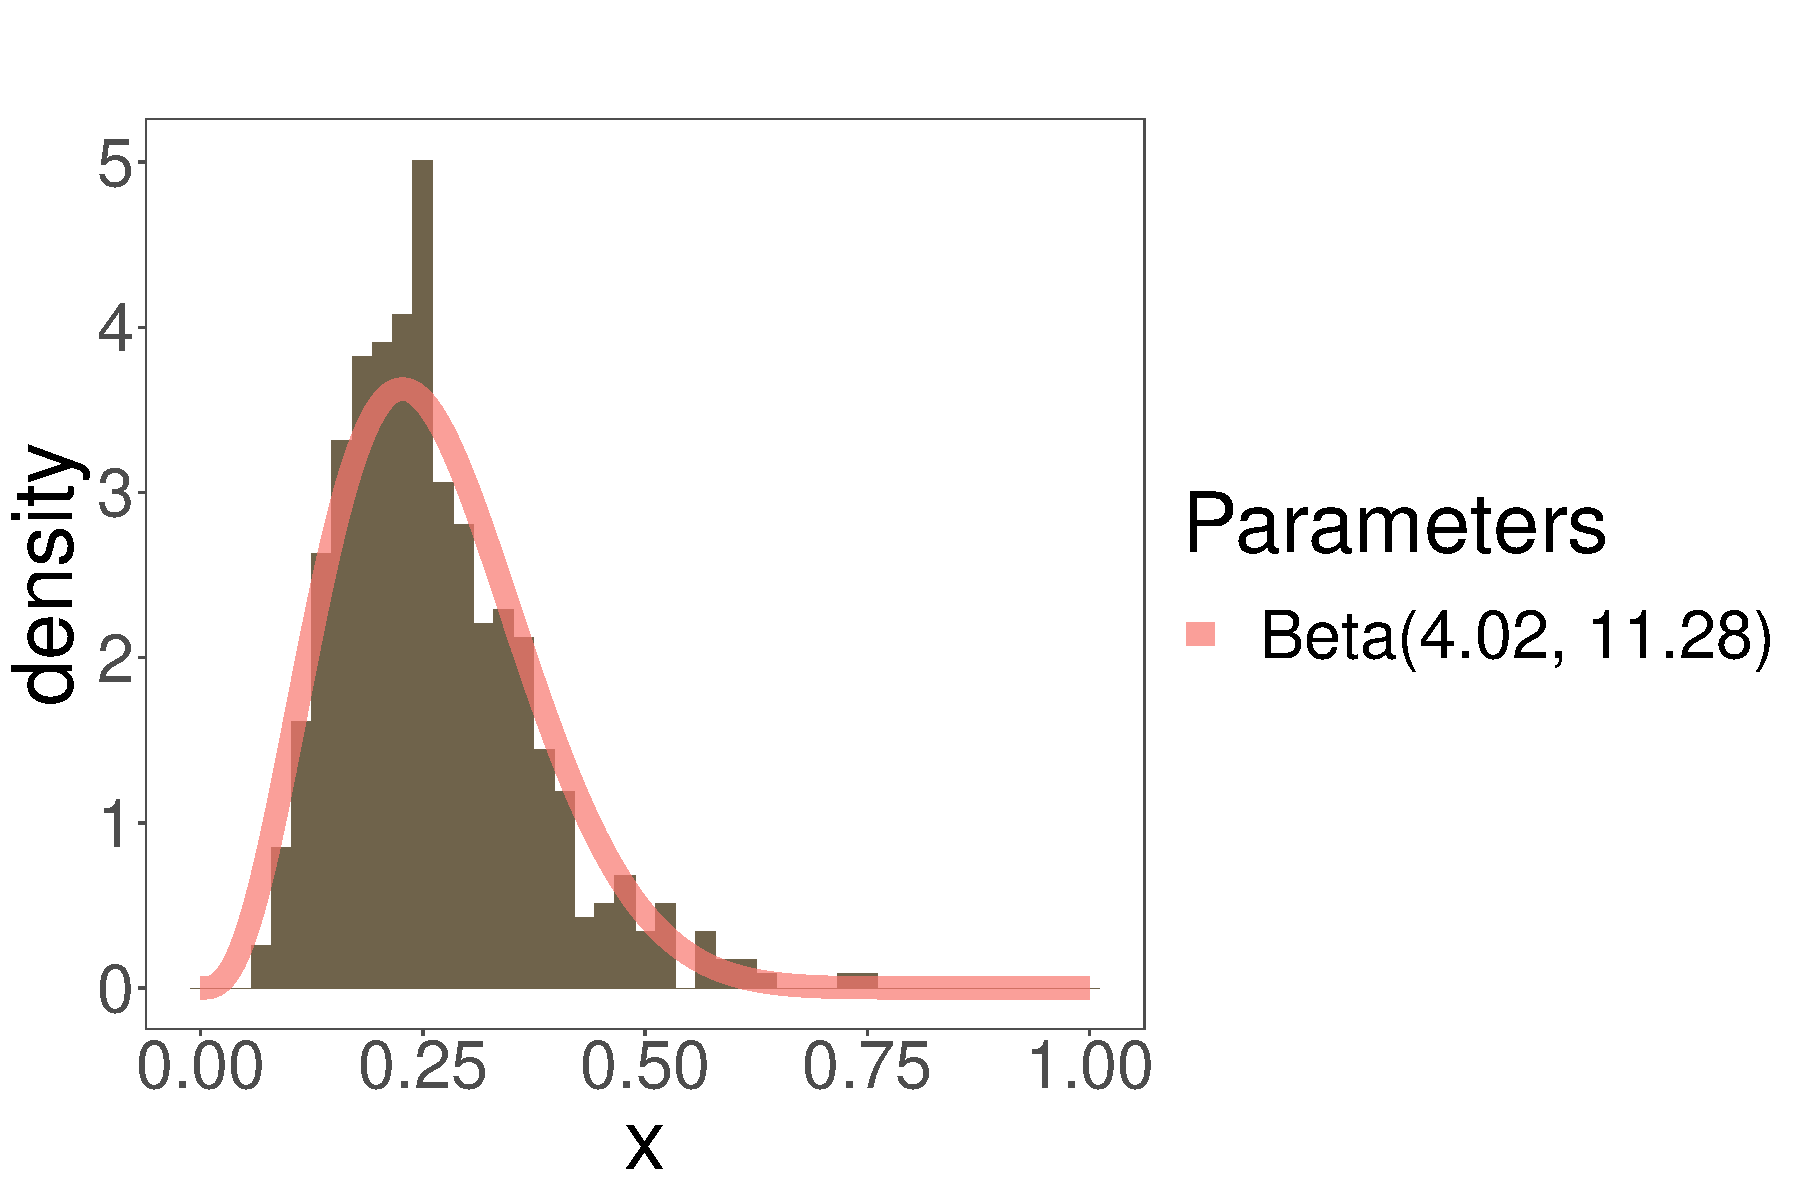
\includegraphics[width = .19\linewidth]{/Histograms/5th_observation/Soybeans_231/histogram_trihedral_5}}
\caption{Histograms of the geodesic distances between trihedral and the pixels of the samples most similar to trihedral}
\label{fig:histograms_alpha}
\end{figure}

\begin{table}[hbt]
  \centering
  \caption{$p$-values from Komolgorov-Smirnov Test}
  \label{tab:pvalues_alpha}
  \begin{tabular}{lrrrrr}
    \toprule
    \textbf{Day} & \textbf{16 May} & \textbf{09 June} & \textbf{03 July} & \textbf{27 July} & \textbf{20 Aug.}\\
                 & \textbf{2016} & \textbf{2016} & \textbf{2016} & \textbf{2016} & \textbf{2016}\\
    \textbf{Sample size} & 1285 & 656 & 449 & 615 & 508\\
    \textbf{$p$-value} & 0.7746 & 0.5734 & 0.3137 & 0.2392 & 0.4158\\
    \bottomrule
  \end{tabular}
\end{table}

Additionally, a separability test was performed in order to assess whether these distances when coming from different images obey the beta distribution for the same set of parameters. From this test the $p$-values shown in the table \ref{tab:pvalues_sep_alpha} were obtained and from these it can be concluded that, at level of 0.05, the only null hypothesis that cannot be rejected is that the selected distances of the last two images obey the beta distribution for the same parameters.

\begin{table}[hbt]
  \footnotesize
  \centering
  \caption{$p$-values from Separability Test}
  \label{tab:pvalues_sep_alpha}
  \begin{tabular}{cccccc}
  \toprule
  & \textbf{16 May} & \textbf{09 June} & \textbf{03 July} & \textbf{27 July} & \textbf{20 Aug.}\\
  & \textbf{2016} & \textbf{2016} & \textbf{2016} & \textbf{2016} & \textbf{2016}\\
  \textbf{16 May 2016} & -- & $7.467 \times 10^{-8}$ & $9.223 \times 10^{-12}$ & $5.159 \times 10^{-21}$ & $1.311 \times 10^{-24}$ \\
  \textbf{09 June 2016} & $7.467 \times 10^{-8}$ & -- & $2.640 \times 10^{-3}$ & $4.551 \times 10^{-4}$ & $1.757 \times 10^{-6}$ \\
  \textbf{03 July 2016} & $9.223\times 10^{-12}$ & $2.640 \times 10^{-3}$ & -- & $4.318 \times 10^{-2}$ & $1.072 \times 10^{-2}$\\
  \textbf{27 July 2016} & $5.159 \times 10^{-21}$ & $4.551 \times 10^{-4}$ & $4.318 \times 10^{-2}$ & -- & $3.642 \times 10^{-1}$ \\
  \textbf{20 Aug. 2016} & $1.311 \times 10^{-24}$ & $1.757 \times 10^{-6}$ & $1.072 \times 10^{-2}$ & $3.642 \times 10^{-1}$ & -- \\
  \bottomrule
  \end{tabular}
\end{table}

\end{document}